\chapter{
2012: A Spatial Capture-Recapture Odyssey
}

\markboth{The End}{}
\label{chapt.final}

\vspace{0.3cm}


\vspace{2in}



\begin{figure}[h!]
\centering
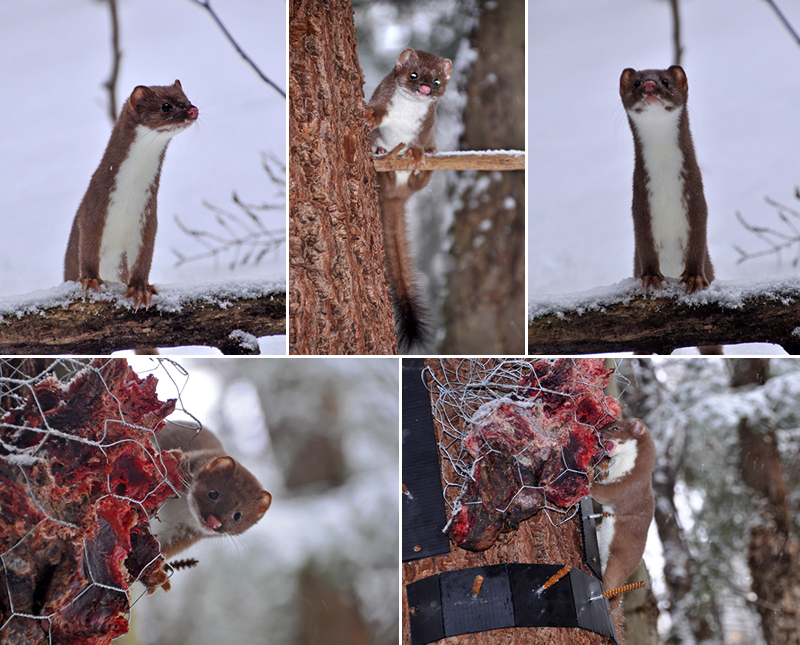
\includegraphics[height=3.5in]{Ch20-Last/Chp20picturearray.jpg}
\caption{
A weasel taking bait on a hair snare.
{\it A Fuller/NYSDEC hair snare study of fishers in
southern NY}, {\it Photo credits: Marty DeLong}
%These are weasels. Cute, blood-thirsty weasels.
%weasels wobble, but they don't fall over
}
\label{last.fig.weasels}
\end{figure}


\begin{figure}[h!]
\centering
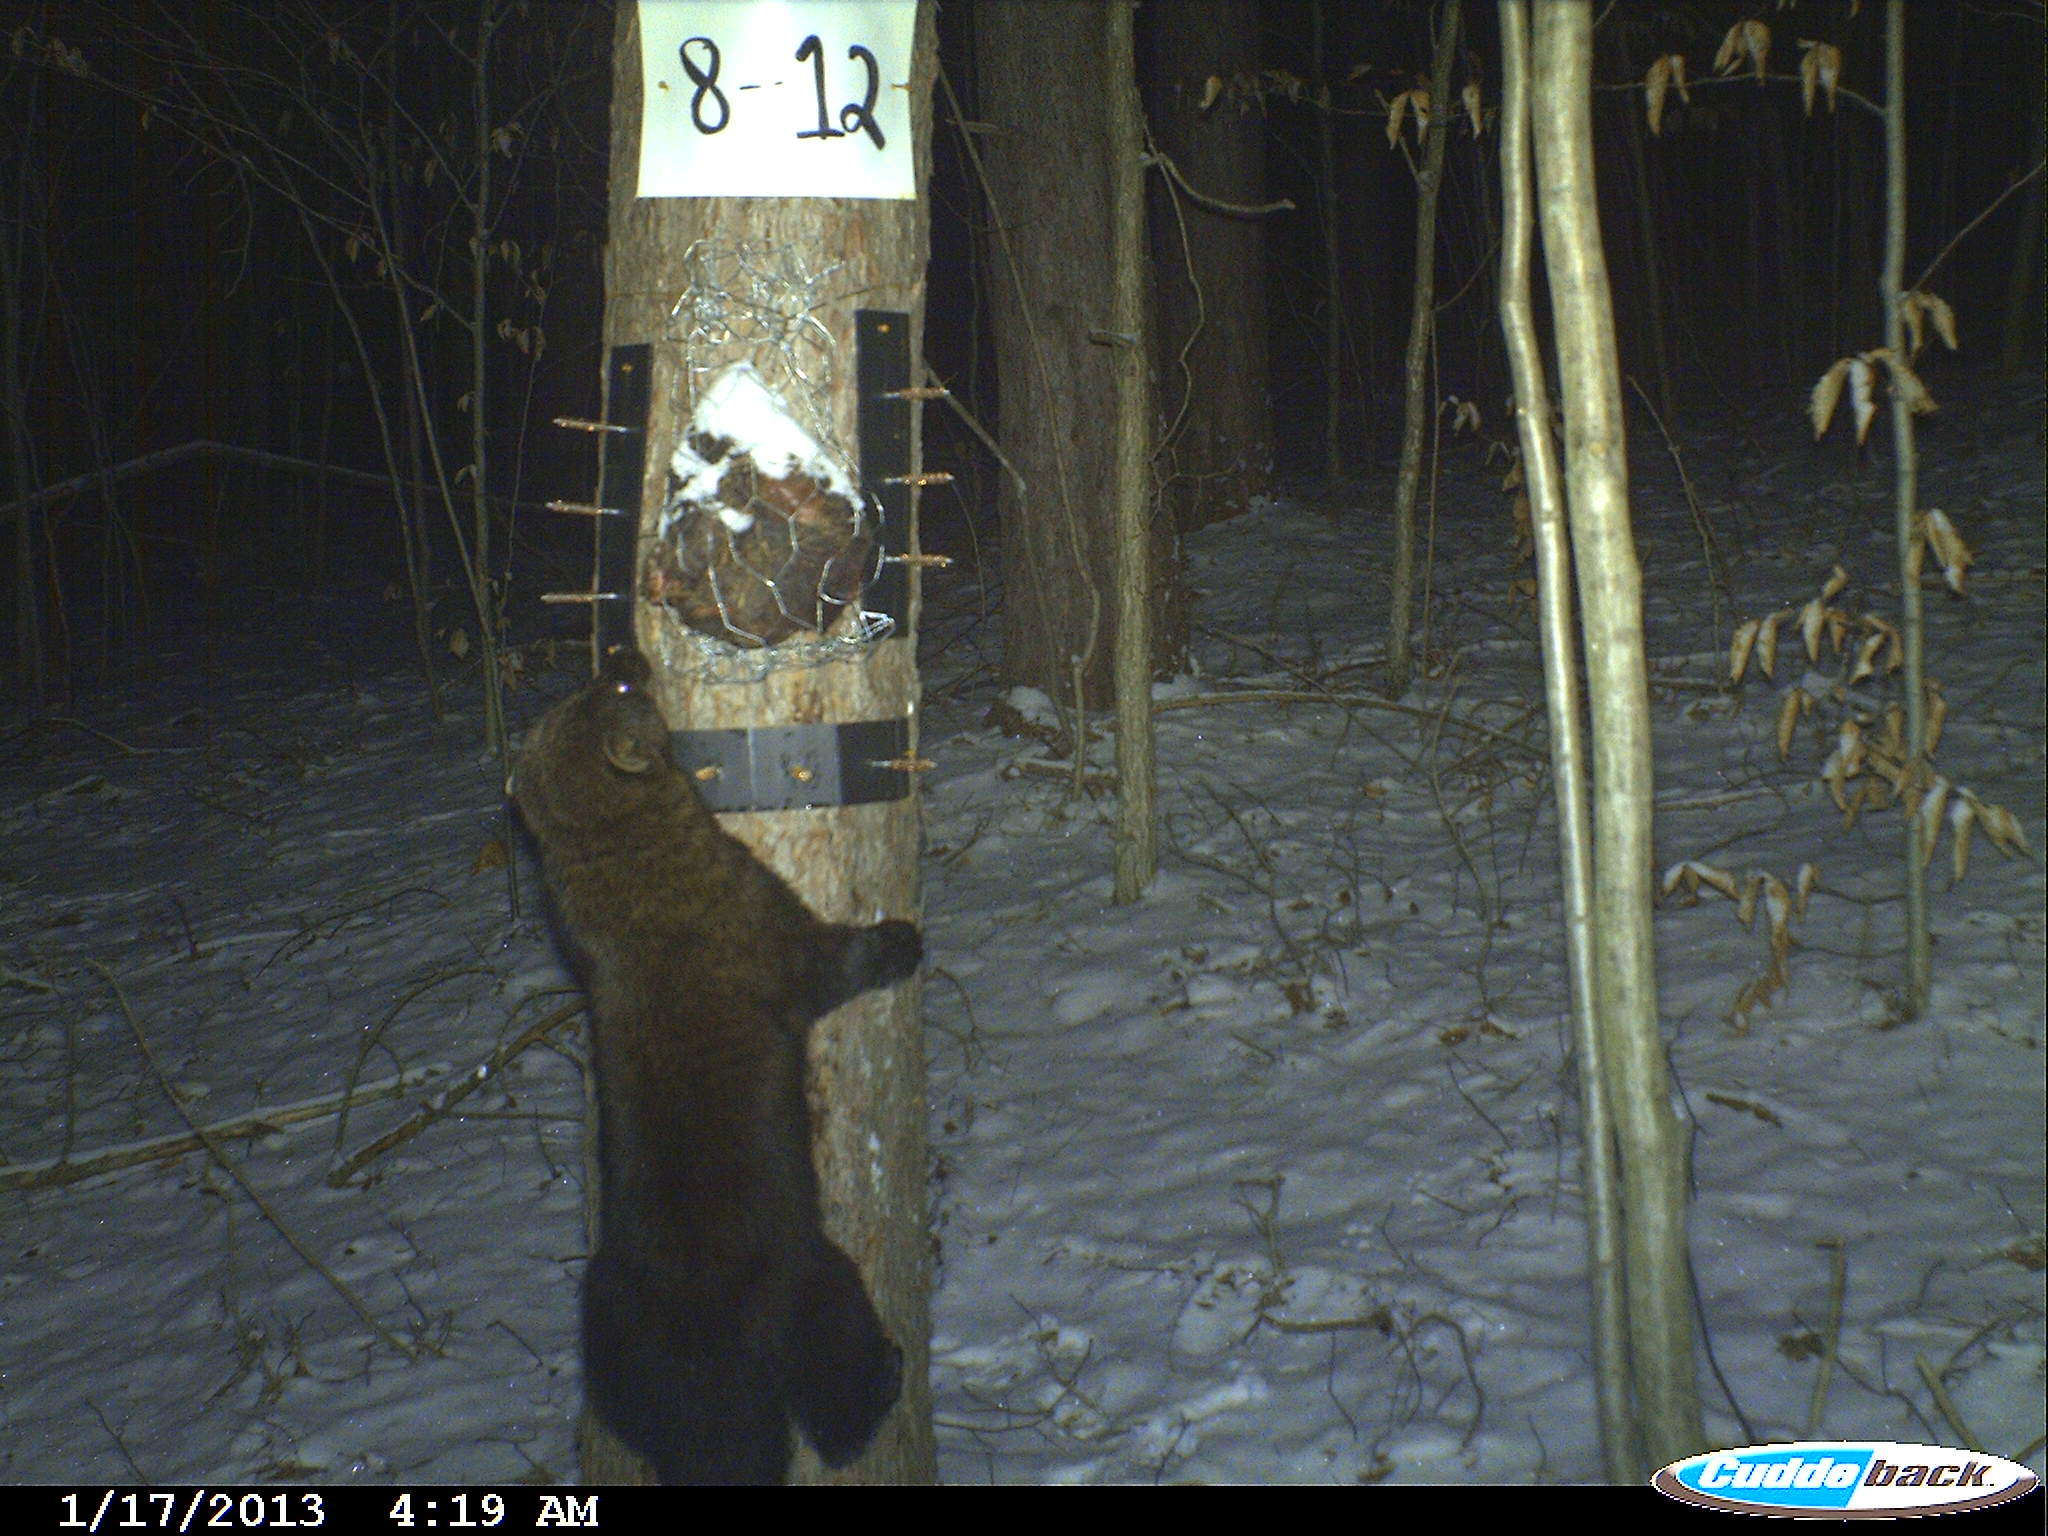
\includegraphics[height=3.5in]{Ch20-Last/fisher.jpg}
\caption{
Fisher assulting tree \# 8-12.
{\it Credit: NYSDEC (New York State Department of Environmental Conservation),
A Fuller/NYSDEC camera trap and hair snare study of fishers in
southern NY}
}
\label{last.fig.fisher}
\end{figure}


\begin{figure}[h!]
\centering
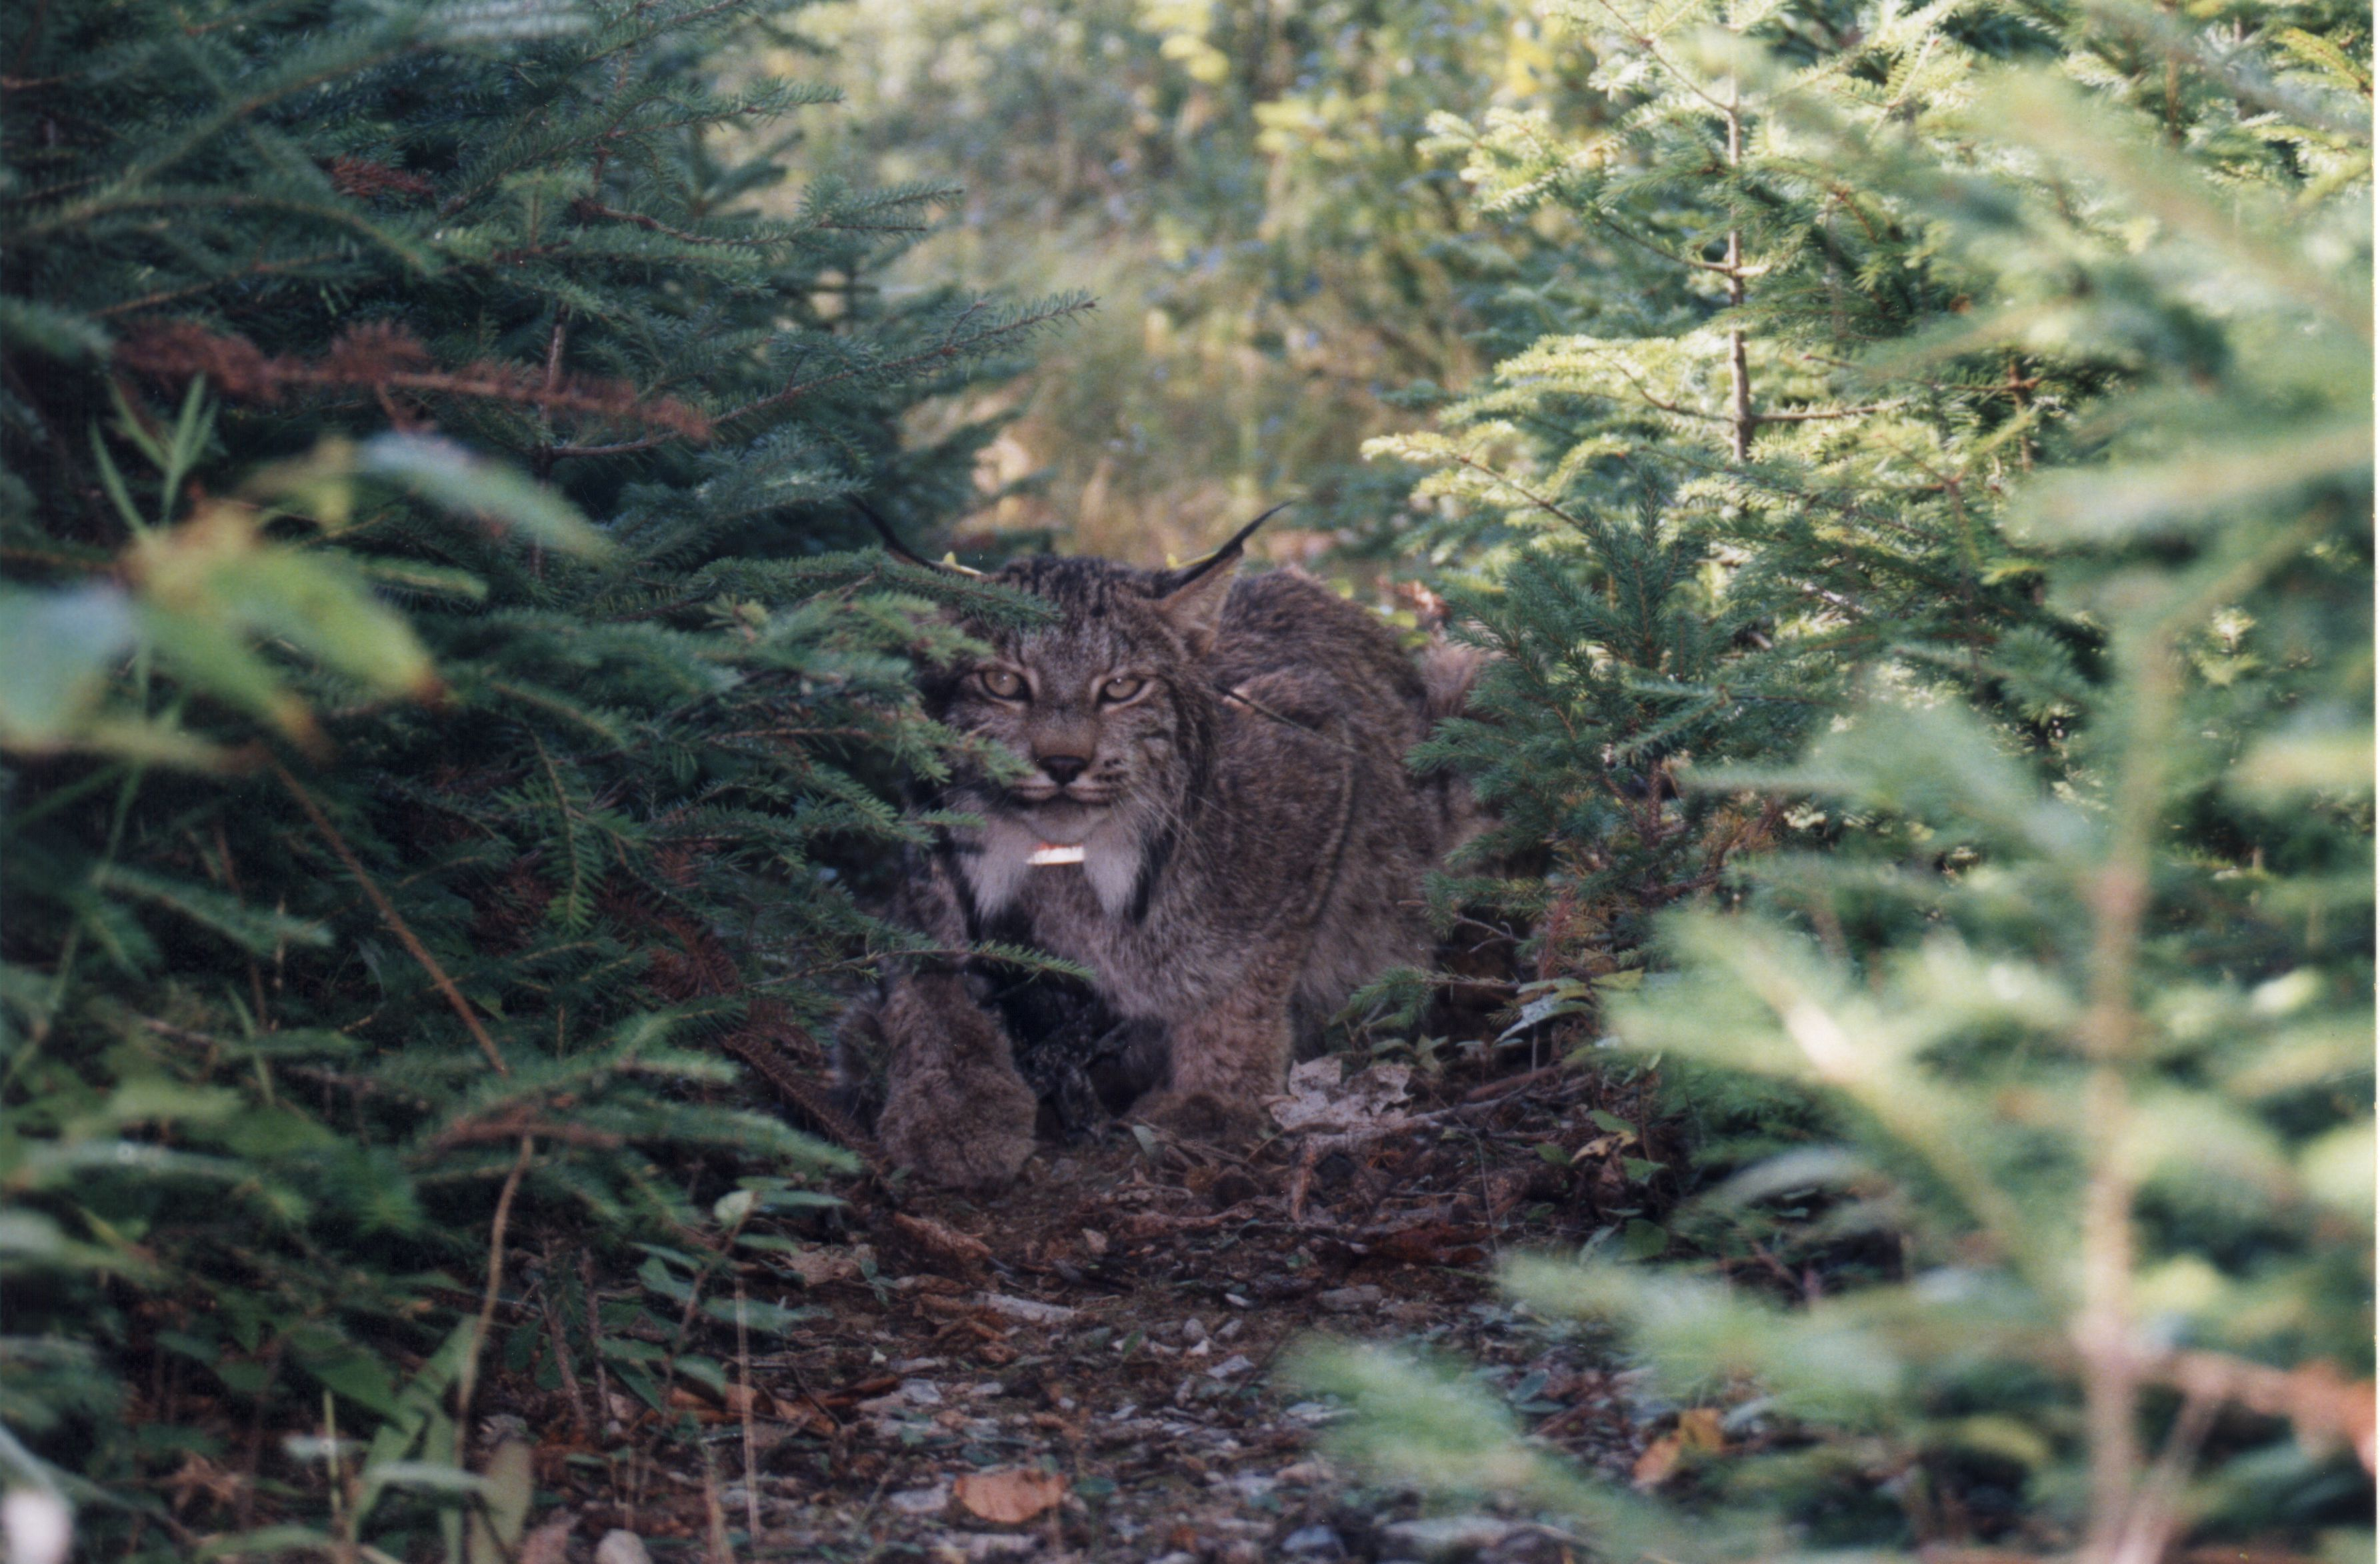
\includegraphics[height=3.5in]{Ch20-Last/lynx.jpg}
\caption{
Canada Lynx, ear-tagged and radio collared, producing high quality
data in the name of science.
{\it Credit: A Fuller, Cornell University} }
\label{last.fig.lynx}
\end{figure}

You've finally made it to the last chapter and we realize it's been a long journey to 
get here (congratulations)! Hopefully this book has provided you with many ideas on how 
to conduct ecological studies, address specific questions that were previously
thought difficult or impossible
to answer before, and given you a solid foundation for carrying out SCR analyses 
on your own. However, we believe this journey is only just beginning and we leave you
now with a few thoughts what we see as the future of SCR methods. 

Let us first consider how we got here. Over a century ago, capture-recapture
methods were first being developed and the study of populations including
spatially varying density was being introduced by Pierre-Simon Laplace and others in France around
1786 (this was of course regarding human population demography, but still, the foundation of how 
we would go on to study animal populations was being laid out). 
The Lincoln-Petersen method was articulated by the 1930s and development of
capture-recapture models began to grow more and more starting in the 1950s. 
Thus, capture-recapture methods became a cornerstone of ecological and wildlife
modeling and analysis. And now, spurred on by the advent of 
new non-invasive technologies like DNA
sampling, camera trapping, acoustic sampling, and other methods,
capture-recapture is more relevant and widely used than ever before
(see also Sec. \ref{last.sec.growth}). These new survey methods allow
researchers to use capture-recapture for species that could not be
studied efficiently even a few years ago, especially those that are
difficult to capture or handle including most felid
(Fig. \ref{fig.last.lynx})
and bear
species, mustelids such as weasels (Fig. \ref{fig.last.weasels}), 
mink and fishers (Fig. \ref{fig.last.fisher}) and many other species. 

So where are we going? With these new sampling techniques, like many commonly used capture-recapture
sampling methods,
auxiliary spatial information about location of capture is collected. As such, classical capture-recapture
models are usually not the right tool for the job of analyzing such data and thus arose the need to develop
models that can directly deal with the spatial information collected in capture-recapture studies. 
The result, as you will have seen in reading this book, was the development of SCR models (starting around
2003 - 2004). We have seen a great increase in the number of papers that use or cite SCR models and to 
articulate the point of where we see SCR usage going in the future, we did a Google Scholar search on 
March 6, 2013 using the terms:
\begin{verbatim}
``spatial capture recapture'' OR ``spatially explicit capture recapture''.
\end{verbatim}
The results, we think, suggest a bright future
for the development and application of spatial capture-recapture
models. Most (but not all) of these papers are about the type of SCR models
discussed in this book although a handful had to
do with other types of spatial analysis as related to
capture-recapture models.
The results from this literature search are shown
in tabular form in Tab. 
\ref{last.tab.cites}.

\begin{table}[ht]
\caption{Google Scholar citations by year based on a search of
\mbox{\tt ``spatial capture recapture'' OR ``spatially explicit
capture recapture''} conducted on March 6, 2013. 
}
\begin{tabular}{lrl} \hline \hline
Time period & Cumulative cites & Cites in year previous \\ \hline
since 2002 & 274 cites & \\
since 2003 & 274 cites &0 articles published in 2002 \\
since 2004 & 271 cites &3 articles published in 2003 \\
since 2005 & 269 cites &2 articles published in 2004 \\
since 2006 & 264 cites &5 articles published in 2005 \\
since 2007 & 261 cites &3 articles published in 2006 \\
since 2008 & 253 cites &8 articles published in 2007 \\
since 2009 & 242 cites &11 articles published in 2008 \\ 
since 2010 & 222 cites &20 articles published in 2009 \\
since 2011 & 176 cites &46 articles published in 2010 \\
since 2012 & 111 cites &65 articles published in 2011 \\
since 2013 & 27 cites &84 articles published in 2012 \\
& &27 published so far in 2013, since March 6
\\ \hline
\end{tabular}
\label{last.tab.cites}
\end{table}

We see rapid growth in the number of citations, 
with growth in citation counts after 2004 fueled by publication of
\citet{efford:2004} and the release of the software DENSITY
\citep{efford_etal:2004}. In 2012 there were 84 articles published and
27 through the first 9 weeks of 2013.

We believe that use and growth of SCR modeling in conservation biology, 
management, wildlife, fisheries, and many other disciplines that we place under
the general umbrella of ecology will only continue. 
This is based on the fact that by explicitly linking the space occupied by individuals with the
spatial location or region of sampling, SCR models 
provide a holistic framework for answering ecological questions
related to the spatial structure of populations -- movement, space
usage, spatial variation in density, landscape connectivity, and other
things. 

And now, after laying out how we got here and where we think SCR models are 
going, we will discuss some of the research areas we see as forthcoming. 
In this book we summarized, synthesized and extended recent
developments of spatial capture-recapture models. The ``big idea'',
if you could distill the whole thing into one idea, is based on
extending closed population models by augmenting them with a point
process model that describes the distribution of individuals
\citep{efford:2004} in space. As a conceptual matter then, the
underlying point locations are regarded as an individual covariate in
the encounter part of the capture-recapture model. In a sense, that is
really all there is to it. But the relevance is much bigger and more
profound because, once we have made space explicit in the model, 
we can think about building population models that embody explicit
spatial processes. 

We talked about some such ideas: landscape connectivity, resource
selection, modeling spatial variation in density. These are all by
themselves profound extensions of the basic capture-recapture method
and they broaden and expand the relevance and utility of
capture-recapture for studying animal populations.
Although we filled almost 600 book pages with SCR methods,
there remains much to be done in the continued development of SCR
models. In the following section, we highlight some emerging topics that show promise or might be in
need of further development. Finally, we end with a few remaining
thoughts on the use of SCR models in the future.



\section{Emerging Topics}

In this book, we provided an overview and synthesis of
capture-recapture methods as known to us around the end of 2012. There
are many emerging topics which we have not covered either because of
lack of technical knowledge, lack of time for satisfactory
development, or lack of a good framework for implementation. Here we
present some of those topics, this is not a complete list by any means,
just a subset of topics that we are currently working on,
or that our colleagues are working on, or that we think 
might make good PhD or Masters projects.



\subsection{Inhomogeneous Point Processes}
\label{last.sec.ipp}

In currently developing work, \citet{reich_etal:2012} propose a model
that accounts for spatial variation in home range density and
potential interactions between individuals' home ranges. This model
lets the activity centers follow an inhomogeneous Strauss process
\citep{strauss:1975}, which allows for spatial variation in the home
range intensity, and includes a parameter that determines the strength
of repulsion between home ranges. The idea is based on the notion
that territorial species would have well defined (and defended) home
range and thus activity centers may be more regular on the landscape
as individuals would avoid one another and/or home ranges would be
less likely to overlap. The development of this work includes a
simulation study, where it was found that properly accounting for
interactions between individuals can provide a substantial improvement
in estimating population size. And thus far, for simulated data
generated with interaction, the usual independence model has a
significant bias for the population size, and generally has larger
uncertainty for the population size than the proposed Strauss process
model.

While the Strauss model is intuitive and shows great potential, it
presents computational challenges. The first challenge is that the
likelihood includes a high-dimensional integral that has no closed
form. To address this issue, \citet{reich_etal:2012} developed an
approximation to the Strauss likelihood which allows for posterior
sampling, extending related work for categorical Markov random fields
\citep{green_richardson:2002,smith_smith:2006}. The second challenge
is that $N$ is treated as an unknown parameter to be updated and hence
$N$ varies and so does the dimension of the likelihood, and thus the
posterior. In this case, the dimension-changing problem can be
overcome by using an auxiliary variable scheme in the Markov chain
Monte Carlo algorithm.
% XX RS: Does that mean you don't use DA?
While the results from an initial analysis of simulated data verifies
that this computational approach leads to reliable inference, there
are still many areas to be explored in using the Strauss model and
other models of clustering.


\subsection{Combining data from different surveys}

In some instances, researchers apply different survey techniques to
the population of interest, because they yield complementary
information. For example, camera trapping is the prime tool for
estimating population size/density and other demographic parameters
for uniquely marked species; genetic surveys can yield additional
information on the genetic diversity and health of a population that
we cannot study using camera traps. At the same time, genetic surveys,
when samples are analyzed to the individual level, also yield spatial
capture recapture data (see Chapt. \ref{chapt.search-encounter}). In
this situation, we have two data sets at hand that carry information
on animal density, and we should be able to get more precise estimates
of density if we combine these two data sets into a single SCR model.

\citet{gopalaswamy_etal:2012mee} developed two approaches to combining
data from different survey types. In the first case, both surveys are
carried out at the same time, so that we can assume that they both
sample the same -- closed -- animal population, i.e., there are no
possible changes in population density between the two surveys. For
camera trapping and genetic surveys, we cannot match records of
individuals between the two data sets. However, models for the
distinct sample methods may share some parameters (e.g., $\sigma$ of
the encounter probability model) and, if the studies were conducted
simultaneously, they share a common population size $N$.

A second approach of using information from one survey in the analysis
of a second survey (that maybe does not yield quite as much data as
the primary survey) is by analyzing your primary data set alone, then
taking the posterior distribution of a parameter both surveys share
and using it as an informative prior distribution in the analysis of
the second data set. \citet{gopalaswamy_etal:2012mee} refer to this as
the stepwise approach, and they implemented this approach by equating
the mean and variance of the posterior distribution of $\psi$ and
$\sigma$ from the photographic survey to the mean and variance of a
beta and a gamma prior for these parameters, respectively, for the
genetic survey. The authors found that this approach produced almost
identical density estimates compared to the combined model approach
described above.

In summary, no matter which approach is chosen, combining data across
surveys can help researchers to obtain more precise population size or
density
estimates, which is especially valuable when dealing with rare and
elusive species like big cats that almost always will produce sparse
individual data sets. 
The paper by \citet{gopalaswamy_etal:2012mee} considers the
situation where we have two SCR data sets, but we can imagine
combining SCR data with other sources of information, such as
telemetry data (see Chapt. \ref{chapt.partialID} and
Chapt. \ref{chapt.rsf} for examples), and possibly opportunistic
observations, although to our knowledge this latter issue has not been
tackled in the context of SCR, yet.


\subsection{Imperfect identification of individuals}

Imperfect identification of individuals can happen in a variety of
ways. In genetic surveys there is usually some probability of
mis-identification of individuals due to genotyping error
(e.g. \citet{lukacs_burnham:2005}). In camera trap survey a different
type of imperfect identification can occur when only the only one
flank of an animal is recorded in a detection event and that imagine
cannot be matched to any of the individuals identified by both
flanks. If that case, we can match single-flank pictures with the same
side flank pictures, but not with opposite side flank pictures and
thus cannot construct definite encounter histories for these
single-flank individuals (a right flank and a left flank picture could
be the same individual, or could be from two distinct
individuals. Finally, in Chapt. \ref{chapt.partialID}, in the context
of mark-resight models, we discussed the case where individuals can
either not definitely be identified as marked or not -- a violation of
a basic mark-resight assumption, and developed an approach to dealing
with the situation where we can always tell if an animal is marked or
not, but we are not always able to ascertain its individual identity.

In non-spatial capture recapture some efforts have been made to
formally deal with misidentification. \citet{stevick_etal:2001}
address this problem by double-sampling to derive an error rate for
genetic identification, and then including this error rate as a known
constant into a Lincoln-Petersen estimator of
abundance. \citet{lukacs_burnham:2005} develop an approach that
includes an additional parameter in the model -- the probability of a
genotype being identified correctly, which is estimated as part of the
model likelihood. \citet{link_etal:2010} developed an approach towards
solving the same problem implemented in a Bayesian framework that
relaxes some of the assumptions of the initial approach.
\citet{yoshizaki_etal:2009} deal with misidentification from camera
trap pictures due to evolving marks (i.e., natural marks that change
over time, such as scars). This situation is different from the
genotyping error one. Here, a change in marks creates a supposedly
`new' individual that can be recaptured several times, while the
original individual is never captured again (its mark is no longer in
the population). In contrast, in genotyping error it is assumed that
misidentification creates a `new' individual that is never observed
again, because each error leads to a new unique
genotype. \citet{yoshizaki_etal:2009} approach this situation
similarly, by including a parameter describing the probability of
correctly identifying an individual upon recapture (the parameter can
also be interpreted as the probability that a mark does not change
between capture occasions). Because of the dependencies between true
and false detection histories (when a `new' individual is created, the
`real' one can no longer be recaptured), the standard multinomial
approach to coming up with a model likelihood does not work and
implementing the model in a maximum likelihood framework is
difficult. The authors instead demonstrate an implementation of the
model based on minimizing a function of the squared differences
between the observed and expected frequencies of the observed capture
histories.

To our knowledge no attempts have been made to deal with
misidentification in an SCR framework. While all of the mis-ID cases
described above require distinct approaches, we believe that there is
one unifying theme to all of them: the location of the un or
potentially mis-identified records and the resulting probabilities of
belonging to certain individuals conditional on their activity
centers. For example, a right flank and a left flank camera trap
picture that are taken at two neighboring camera traps are more likely
to belong to the same individual that a right and a left flank picture
taken at cameras at opposing ends of the trap array, especially if
animal movement is smaller than the extent of the trap array; an
unidentified record of a marked individual in a mark-resight survey is
more likely to belong to a marked individual whose activity center is
close by, than to an individual whose activity center is located far
away; and so forth. Formally developing misidentification models
should be a focus for future SCR model development.

\begin{comment}
\subsection{Three dimensional space}

Throughout this book we have treated space as
two-dimensional, meaning that activity centers are assumed to occur on
the real plane. This approximation of reality is reasonable for many
terrestrial species, but aquatic organisms, especially marine animals
move about in three-dimensional space. Treating space as
three-dimensional could also conceivably be useful in studies of
flying organisms, aquatic organisms,
or species that use multiple strata of tall forests; however, we
suspect that two dimensional models of space should suffice in such
contexts. Regardless, a three-dimensional view of space requires that
activity centers $\bf s_i$ are indexed by
$x,y,z$ coordinates. In theory, this presents no problem whatsoever. In
practice, estimation based on integrated likelihood methods must
involve a three-dimensional integration. This will clearly be more
computationally demanding, but it should be possible using packages
such as {\tt R2Cuba}.
\end{comment}

\subsection{Gregarious species}

One of the key assumptions of the SCR models that we described
throughout this book is that the activity centers are independent of
one another. There are good biological reasons why this shouldn't be
the case, and one of those is when species associate with one another
as a pair, or family group.
Even species regarded as solitary often join family
groups for some portion of their life cycle. We believe that general
models for non-independence of activity centers can be developed (see
Sec. \ref{last.sec.ipp} above).

There are two consequences of individuals that exist as a pair or
group. For one, the detections are not independent. A trap that
catches one of the individuals is likely to capture others in the
group.
% XX RS: Didn#t Robin also show that this kind of clustering doesn't really have an effect on estimates, at least for family groups up to some size that I do't remember...
The other consequence is that the activity centers ${\bf s}_{i}$
should appear clustered or, in fact, completely redundant in some
cases. A possible way to account for this is to change our definition
of ${\bf s}_i$ from the location of an individual's activity center,
to the location of a group's activity center
\citep{russell_etal:2012}. Ideally, to accommodate unknown group size,
the SCR model would be expanded to include a submodel for group size,
so that formal estimation of both group density and group size would
be possible.



\subsection{Design}

model-based design is huge. Design of SCR studies is naturally
amenable to standard considerations of model-based spatial design
\citep{muller:2007} which we introduced back in
Chapt. \ref{chapt.design}. Clearly more work can be done on this
problem and we think at some point not too far into the future, there
will be general-purposes platforms for building capture-recapture
sampling plans.
A number of specific design problems require some
investigation...... designing large landscape scale capture-recapture
studies where uniform coverage with traps cannot be achieved, needs
to be done.
Design in the context of modeling spatial variation in
density..... and the effect on design of having telemetry or other
auxiliary data.


\subsection{Acoustic models}

At the 2012 ISEC Borchers talked about a number of interesting 
developments and applications of acoustic models. Multiple observers
``triangulating'' on a source, and some other things.

\subsection{Single Catch Traps}

In Chapt. \ref{chapt.poisson-mn} we talked about multinomial models in
which encounter of individuals is independent for all
individuals. this is the multi-catch type of device in which traps
never fill-up, but an individual can only be caught in one trap. We
suggested (following that of \citet{efford_etal:2009euring}) that the
multi-catch, independent multinomial model, could be used for ``single
catch'' traps (traps that hold a single individual or ``fill up'') and
that bias associated with mis-specifying the model would be low under
certain conditions (i.e., when the proportion of occupied traps is
low).


As discussed in Chapt. \ref{chapt.poisson-mn}, 
sec. \label{poisson-mn.sec.singlecatch},
we recognize that the {\it time} of capture of an
individual in any trapping interval will affect the encounter
probability of subsequently captured individuals. Thus if 
the order of capture was known, then this information could be 
used to write the likelihood. However, the order of capture
is almost never known, but we think that if you could consider all
possible orderings, then you would have a close approximation to the
likelihood. All possible orderings of capture couple would be quite
computation intense and so we are working on a solution that selects
an arbitrary ordering the captures as a practical approximation to the
single-catch process. This will hopefully lead to a formal model
for the the single catch trap problem.


\subsection{Model Fit and Selection}

Evaluation of model adequacy or ``fit'' is an important part of any
applied analysis. In Chapt. \ref{chapt.gof}, we offered up a number of
ideas based on standard considerations and adapated and applied them
to SCR models. However, these ideas have not been widely applied, or
evaluated, and much work needs to be done. In particular, some basic
analysis of their power under meaningful alternatives would increase
their relevance and possibly lead to insights for devising better
methods. This applies to both Bayesian and likelihood-based methods,
for which there are even fewer published applications of
goodness-of-fit assessment.

Similarly, we discussed model selection strategies using more-or-less
conventional ideas based on AIC/DIC, and model indicator variables
using the \citet{kuo_mallick:1998} method. Calibration of these
methods under alternatives is needed, along with some analysis of
sensitivity to density estimates to misspecification of certain model
components.


\subsection{Dynamics}

%Dynamic point processes:
%Movement, Dispersal, Migration,
%Transience.

We briefly discussed the topics of dispersal,
transience, and migration in Chapt. \ref{chapt.open} and sketched out
a few ideas for allowing the point process that describes the activity centers
to be dynamic. %other chapters? RSF?
Temporary emigration and transiency are two topics where
a significant amount of work has been accomplished in non-spatial closed and open capture-recapture
models \citep{kendall_etal:1997, pradel_hines:1997, hines_etal:2003,
clavel_etal:2008, gilroy_etal:2012,chandler_etal:2011}.
Additionally, models for dispersal (e.g., \citet{clobert_etal:2001,
ovaskainen:2004, ovaskainen_etal:2008} and 
and movement (e.g., \cite{jonsen_etal:2005, johnson_etal:2008b,
mcclintock_etal:2012}) have received quite a bit of attention and development in
ecology.

With the formulation of SCR models, the framework is already in place to provide
a formal incorporation of the movement dynamics governing the processes
of dispersal, emigration, and transiency. 







\subsection{Miscellaneous topics}

Models for unmarked or partially marked individuals integrated with RSF data from telemetry

Occupancy and counts data + SCR data (AOAS and Sollmann et al.)

Spatial genetics -- can use SCR to study gene flow, related things....

SCR on dendritic networks (streams and trails).


\section{The Future of SCR}

Everything in ecology is spatial, and now so too are capture-recapture
models. We imagine that as SCR models continue to be developed and
extended, their use will continue to grow as well. While there are not
a huge number of applications of SCR models right now, we showed that
their use has expanded rapidly based on simple scitation counts. 

Considering the number of citations as an ordinary population (without
spatial context!), we used these data to make a projection of the
number of published articles that involve SCR methods into the future.
We fitted an exponential growth curve to these data and estimate the
annual rate of growth to be 33.4\%, accounting for the partial year of
data observed in 2013.
% XXXX RC: I would get rid of the predictions.
% Andy sez: is this too pretentious? haha. Probably is....

% Beth says: yeah, I agree with Richard. I showed Jason
%"the graph and he thought it was cool, but then he said,
%"it kind of seems a bit much, a little to pretentious"

We used the model to project the number of
publications that involve SCR models into the future
(Fig. \ref{last.fig.expgrowth}). This includes the observed data
(solid circles) (omitting the partial year 2013) and projections up to
2020. We conclude that the future of SCR is bright, with 800 or 900
publications predicted to occur in 2020. While this is a long time in
the future to be predicting based on an exponential growth model, we
can do some model checking along the way, as the prediction of 85 SCR
publications in 2013 and 119 in 2014 can be assessed in short order,
giving us some short-term feed-back on the state of the system. Of
course, this model is missing some important things. One of those is
carrying capacity. The model predicts $>800$ publications in 2020, but
there may not be that much capacity to do capture-recapture studies!


\begin{figure}[ht]
\centering
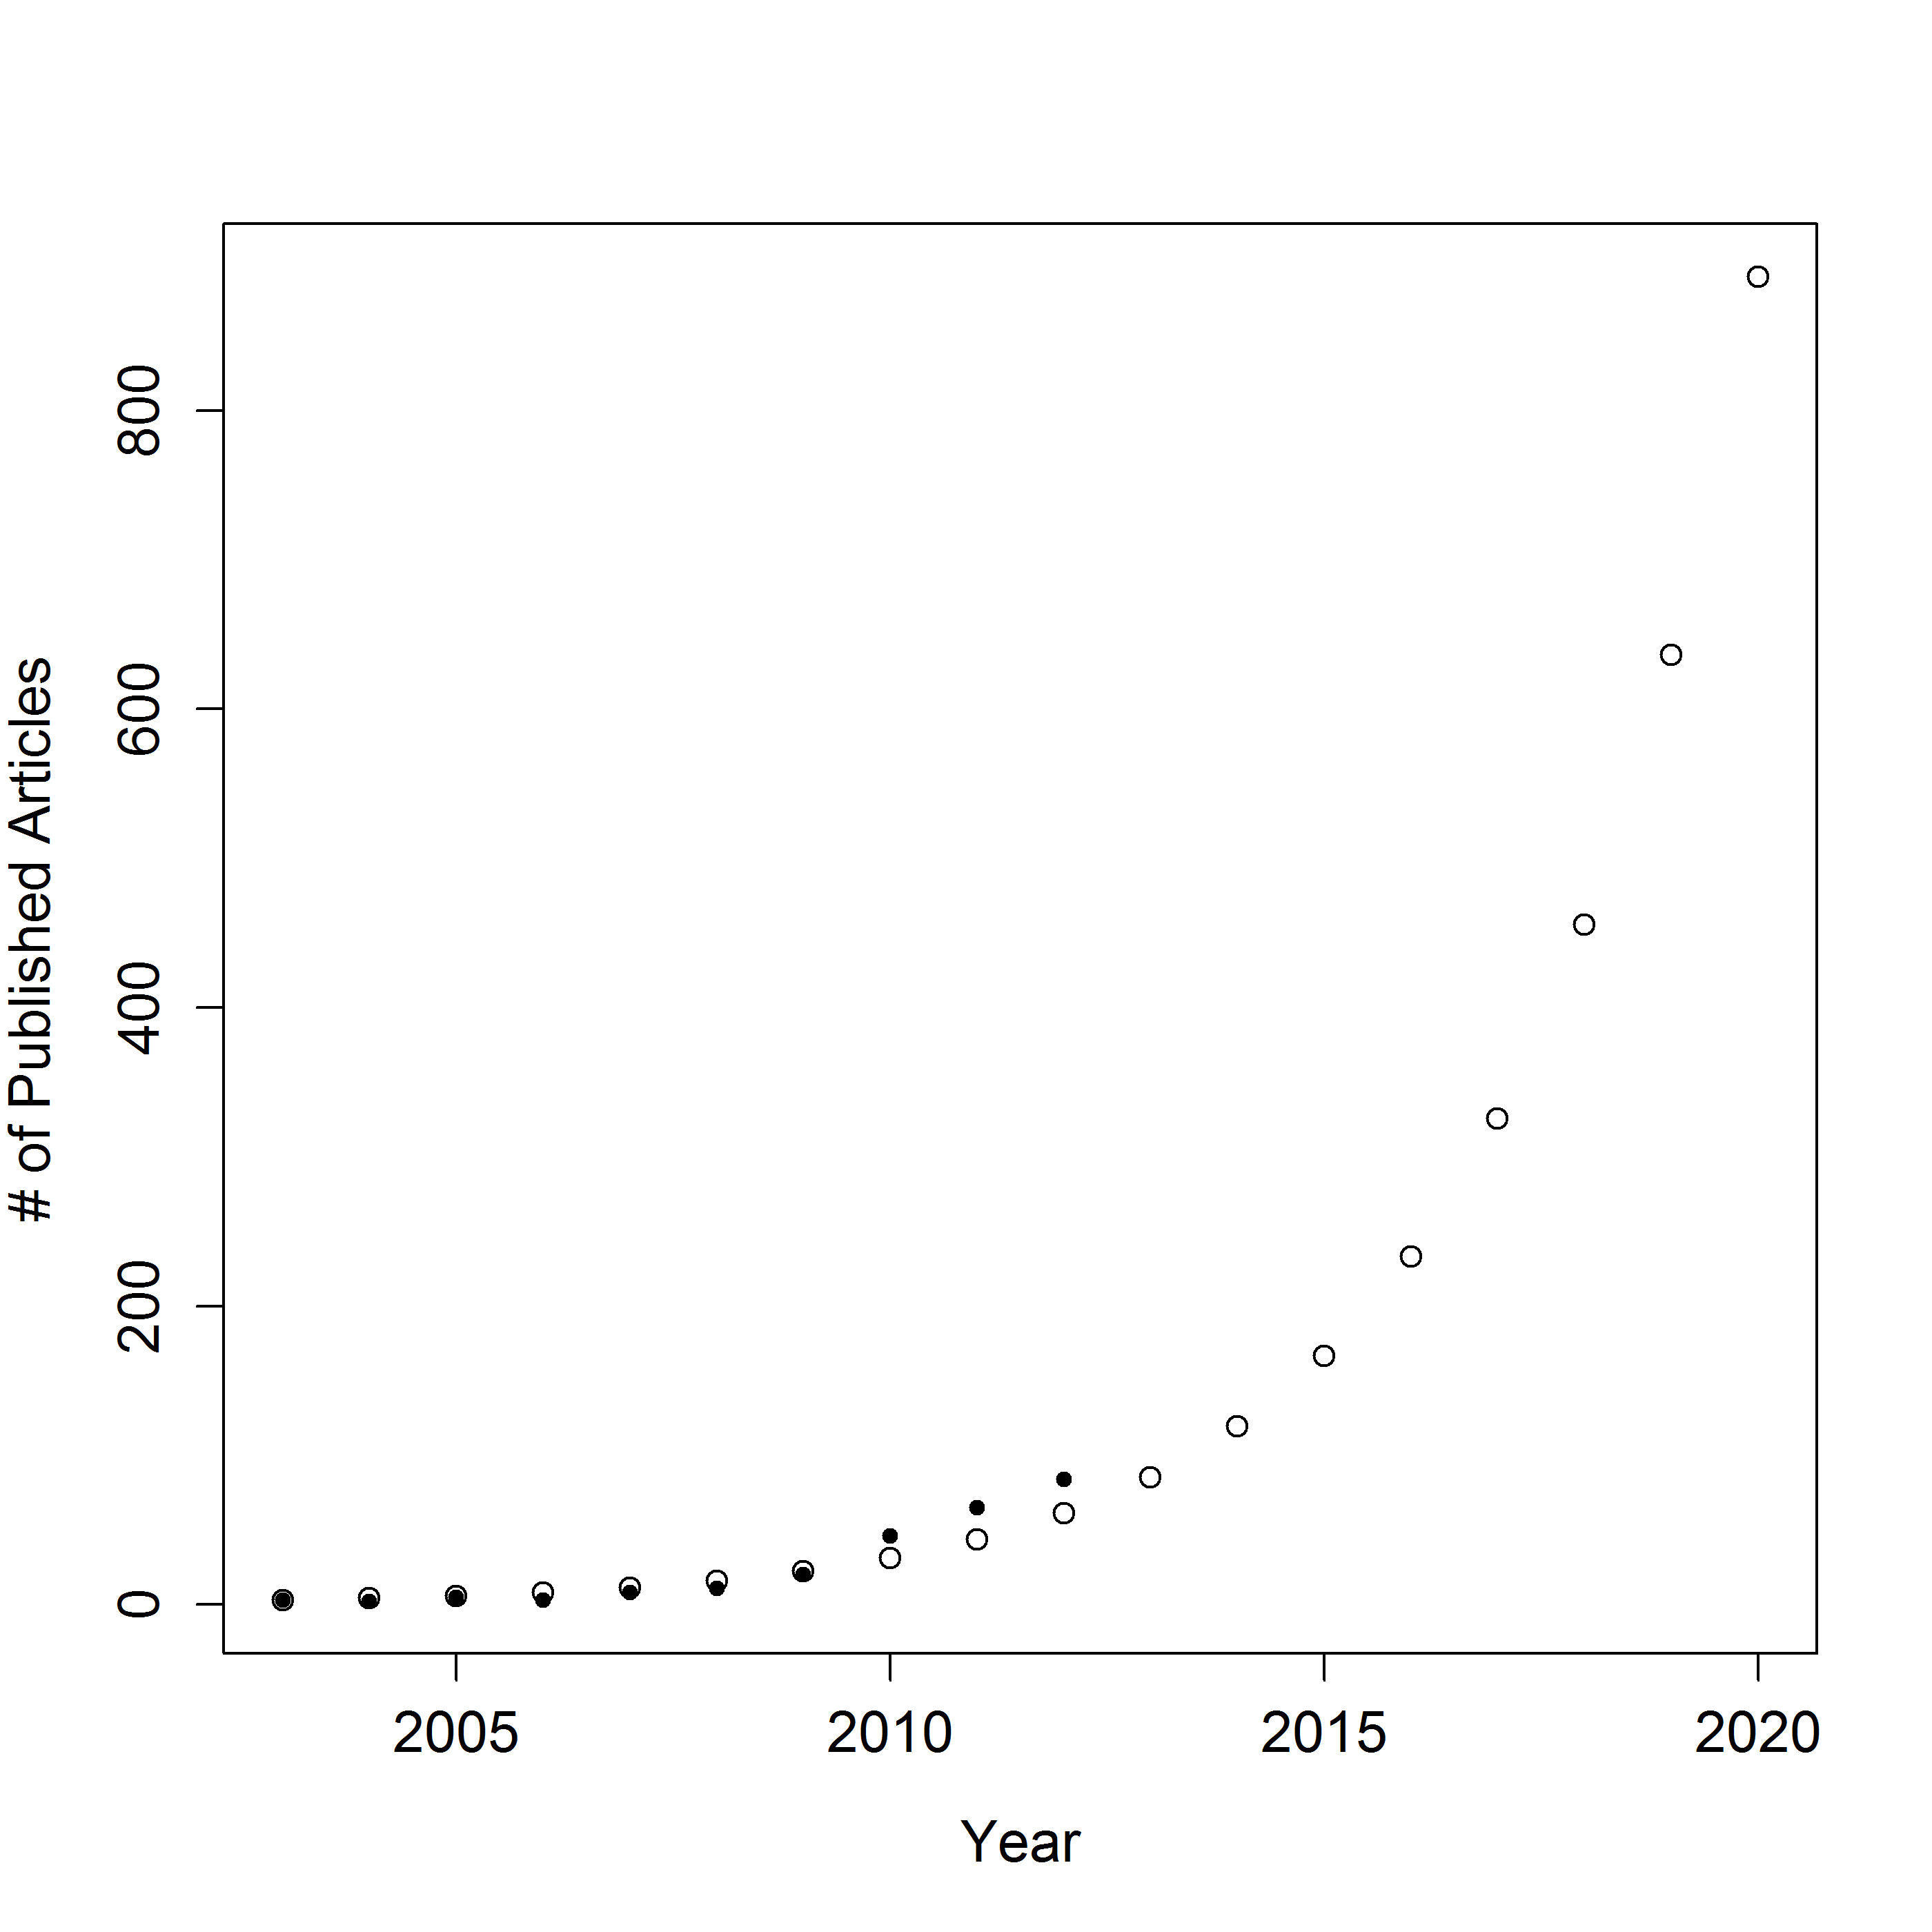
\includegraphics[width=4in,height=4in]{Ch20-Last/exp_growth.png}
\caption{
exponential growth projection of population size of published articles
that involve SCR models.
}
\label{last.fig.expgrowth}
\end{figure}





Historically the main use of capture-recapture was to obtain population
size estimates, but
SCR models allow you to address basic and applied questions of
population ecology from individual encounter history data. Problems
having to do with movement, space usage, landscape connectivity, and
how individuals organize themselves in space.

We envision that SCR models will be useful in helping
ecologists ``do science'' by developing explicit models of spatial
processes, space usage, connectivity, etc., using ordinary, cheap, and
easy to obtain individual encounter history data. Much work needs to
be done to improve computational feasiability, to address many
technical or methodological holes in the literature (see previous
sections), and to make these methods accessible to practitioners.







